\documentclass[12pt,onecolumn,a4paper,fleqn]{article}
\usepackage[top=1in, bottom=1in, left=0.75in, right=0.75in]{geometry}
\usepackage{epsfig,graphicx,subfigure,amsthm,amsmath}
\usepackage[table,xcdraw,svgnames]{xcolor}
\usepackage{setspace}
\usepackage{mathtools}
\usepackage{fancyhdr}
\usepackage{sidecap}
\usepackage{tikz}
\usepackage{pgfplots}
\usetikzlibrary{decorations.pathreplacing}
\usepackage{relsize}
\usepackage{color,xcolor}
\usepackage[framed,numbered]{matlab-prettifier}
\usepackage{float}
\usepackage{enumerate}
\usepackage{booktabs}
\usepackage{setspace}
\usepackage{datetime}
\usepackage{xepersian}


\settextfont[Path=fonts/,BoldFont={ZarBd.ttf},BoldFeatures={Scale=0.9}]{BZar.ttf}

%\DeclarePairedDelimiter\ceil{\lceil}{\rceil}
%\DeclarePairedDelimiter\floor{\lfloor}{\rfloor}

%\definecolor{vgreen}{RGB}{104,180,104}
%\definecolor{vblue}{RGB}{49,49,255}
%\definecolor{vorange}{RGB}{255,143,102}


% title page template
\newcommand{\heading}[1]
{
	\begin{center}
		\begin{huge}
			\textbf{
				به نام خدا\\
			}
		\end{huge}
		
		\vspace*{1.5cm}
		
\includegraphics[scale=0.9]{source/sharif_logo.png}\\
		\vspace*{0.5cm}
		\begin{Large}
			\textbf{
				دانشگاه صنعتی شریف\\
				\vspace*{0.25cm}
				دانشکده مهندسی کامپیوتر\\
			}
		\end{Large}
		\vspace*{3cm}
		\begin{huge}
			\textbf{
				آزمایشگاه معماری کامپیوتر\\
				\vspace*{0.75cm}
			}
		\end{huge}
		
		\begin{Large}
			\textbf{
				آزمایش ششم:\\
				#1\\
			}
		\end{Large}
		
		\noindent\rule[1ex]{\linewidth}{1pt}\\
		\vspace*{0.5cm}
		\begin{table}[H]
			\centering
			\begin{tabular}{|c|c|}
				\hline
				\multicolumn{2}{|c|}{\textbf{اطلاعات تیم}}
				\\ \hline
				\textbf{نام اعضا} & \textbf{شماره دانشجویی}
				\\ \hline
				متین داغیانی & 98106456
				\\ \hline
				بردیا محمدی & 98171104
				\\ \hline
				محمدجواد هزاره & 98101074
				\\ \hline 
			\end{tabular}
		\end{table}
		\begin{Large}				
			\vspace*{0.75cm}
			\textbf{
				پاییز 1400
			}
		\end{Large}			
	\end{center}
}

\pagestyle{fancy}
\fancyhf{}
\rhead{\textbf{آزمایشگاه معماری کامپیوتر}}
%%--------------------[should change]---------------------
\chead{\textbf{گزارش آزمایش ششم}}
%%--------------------[should change]---------------------
\lhead{\textbf{\nouppercase{\rightmark}}}
\cfoot{({\thepage})}
\renewcommand{\headrulewidth}{1pt}
\renewcommand{\footrulewidth}{1pt}
\renewcommand{\sectionmark}[1]{\markright{#1}}
\renewcommand{\subsectionmark}[1]{\markright{#1}}
%\newdateformat{monthyeardate}{%
%	\monthname[\THEMONTH], \THEYEAR}

\onehalfspacing
\begin{document}
	%%% title pages
	\large
	\begin{titlepage}
		\heading{کنترل توسط برنامه ذخیره شده در حافظه}
		\thispagestyle{empty}
	\end{titlepage}	
	\pagebreak
	
	%%% contents page
	\tableofcontents
	\thispagestyle{empty}
	\pagebreak
	
	%%% figures page
		\listoffigures
		\thispagestyle{empty}
		\pagebreak
	
	%%% main document
	\section{هدف آزمایش}
	هدف از این آزمایش آشنایی با نحوه واکشی و اجرای دستورات از حافظه دستور در پردازنده است. برای پیاده سازی لام است تا فرمانهای لازم جهت کنترل مدار را از برنامه ذخیره شده در \lr{EPROM} واکشی کرده و سپس اجرا کنیم. بدین جهت مدار زیر را به واحد چریان داده طراحی شده در آزمایش پنجم اضافه می کنیم.
	\begin{figure}[H]
			\centering
			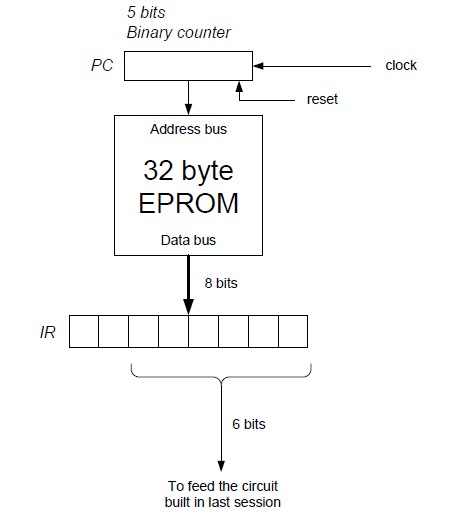
\includegraphics[width=0.68\textwidth]{source/1.jpg}
			\caption{بلوک دیاگرام سیسیتم}
			\label{fig:1}
	\end{figure}
	همان طور که در تصویر بالا مشخص است، این سیستم شامل یک \lr{PC}   پنچ بیتی است که آدرس دستور بعدی در حافظه را مشخص می کند. هم چنین دستورات برنامه در حافظه ذخیره شده اند. پس از واکشی دستور بعدی وارد رجیستر \lr{IR} که ورودی واحد جریان داده است می شود. مطابق آزمایش پنچم، برای تعیین هر دستور به 6 بیت نیاز داریم که در شکل نیز معلوم است. نمای کلی مدار پیاده سازی شده در ادامه آمده است.
	\begin{figure}[H]
				\centering
				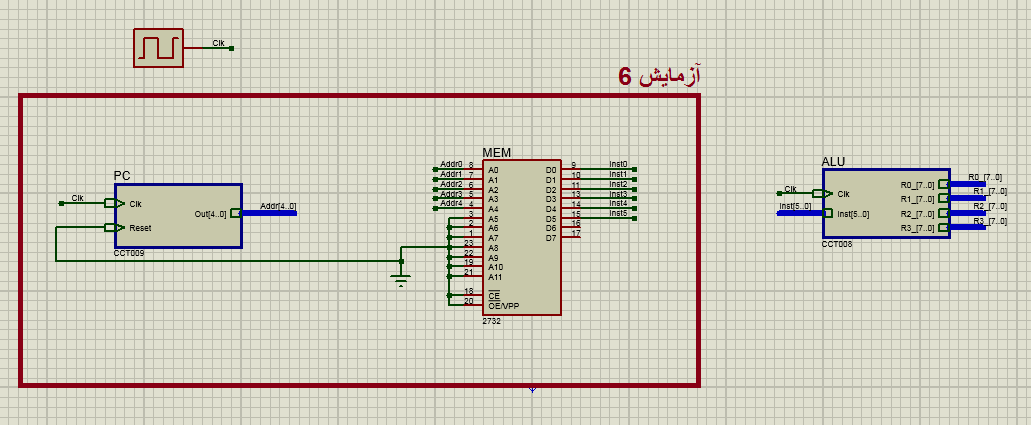
\includegraphics[width=0.68\textwidth]{source/2.png}
				\caption{نمای کلی سیستم پیاده سازی شده}
				\label{fig:2}
	\end{figure}
	\section{مراحل طراحی و پیاده‌سازی مدار}
	\subsection*{ماژول‌های مورد نیاز و شروع به کار مدار}
		همانطور که در شکل \ref{fig:1}  مشخص است، برای پیاده سازی سیستم فوق به یک شمارنده باینری 5 بیتی نیاز داریم، به طوری که در هر واحد کلاک، یک واحد به آن اضافه شود تا دستور بعدی در حافظه دستورات را مشخص کند. به علاوه به یک \lr{EPROM} با 5 خط آدرس نیاز داریم. طول هر واحد حافظه  1 بایت است که در نتیجه ظرفیت نهایی برابر با 32 بایت می شود. 
	\subsection{ماژول \lr{PC}}
		\begin{figure}[H]
					\centering
					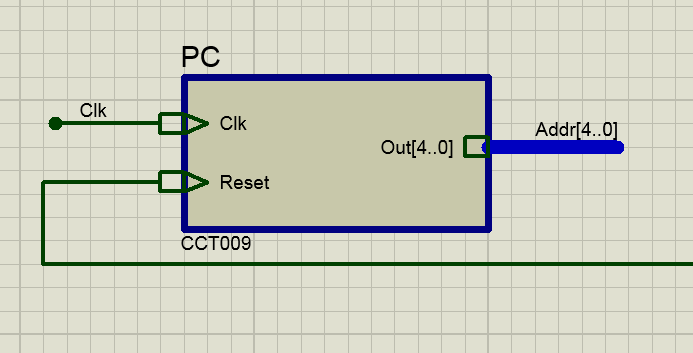
\includegraphics[width=0.68\textwidth]{source/3.png}
					\caption{ماژول شمارنده 5 بیتی}
					\label{fig:3}
	\end{figure}		برای پیاده سازی این ماژول از معماری \lr{ripple} استفاده شده است. به طور دقیق تر، شمارنده فوق از 5 فلیپ فلاپ \lr{JK} تشکیل شده است، به طوری که خروجی \lr{Q} هر یک مشخص کننده یک بیت از خروجی مدار است(خروجی های \lr{Out}). هم چنین ورودی ها \lr{J} و \lr{K} تمامی آن ها به ورودی 1 متصل هستند تا هر کدام در وضعیت \lr{Toggle} قرار گیرند. 
	\begin{figure}[H]
						\centering
						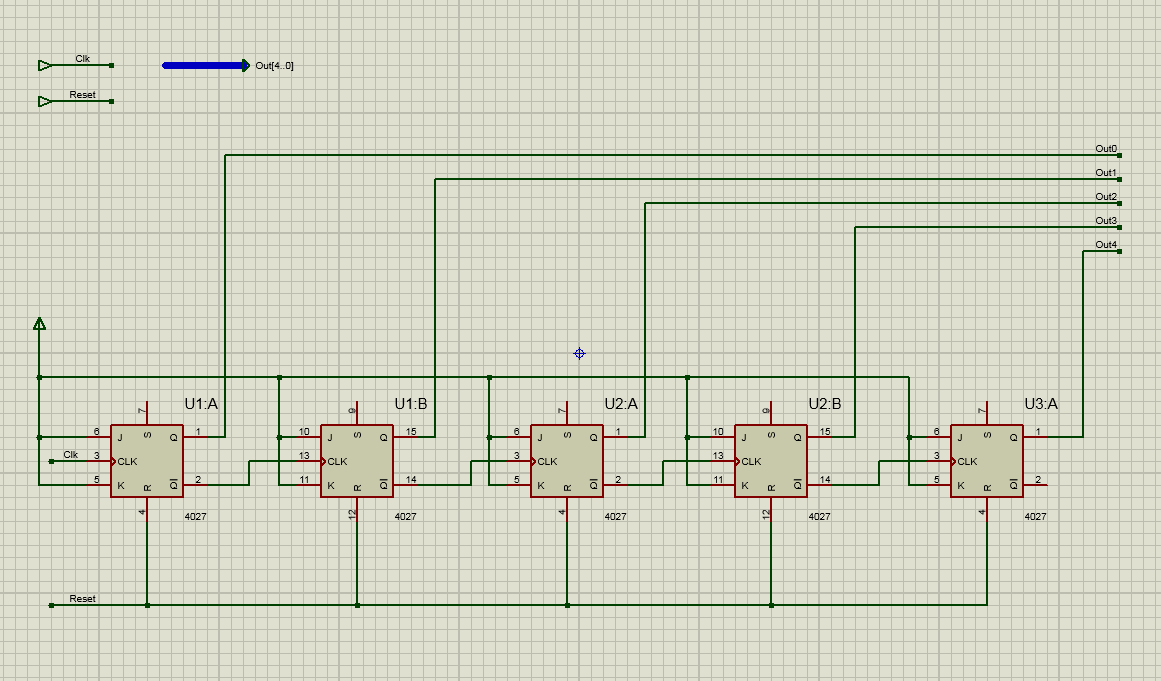
\includegraphics[width=0.68\textwidth]{source/4.png}
						\caption{نمای داخلی ماژول شمارنده 5 بیتی}
						\label{fig:4}
	\end{figure}
	
	\subsection{ماژول \lr{Memory}}
	برای پیاده سازی این ماژول از تراشه آماده 2732 استفاده شده است. این تراشه یک \lr{Erasable Programmable ROM} است که از 12 خط آدرس و 8 خط خروجی تشکیل شده است. با توجه به نیاز این آزمایش، تنها از خطوط آدرس \lr{A0 - A4} و خطوط خروجی \lr{ِD0 - D5} مورد استفاده قرار گرفته اند. لذا تمامی خطوط آدرس دیگر به ورودی صفر متصل هستند. در شکل زیر این ماژول را ملاحظه می کنید:
	
	\begin{figure}[H]
							\centering
							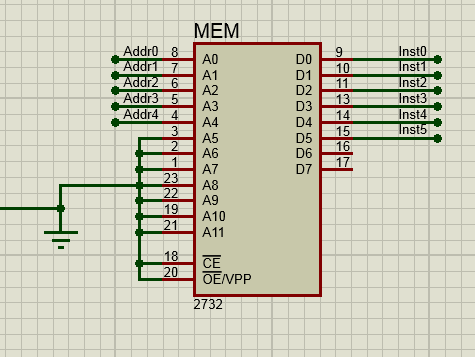
\includegraphics[width=0.68\textwidth]{source/5.png}
							\caption{ماژول حافظه دستورات}
							\label{fig:5}
	\end{figure}
	برای برنامه ریزی محتوای این ماژول، از فایل \lr{memroy.bin} که هم سطح فایل پروژه واقع است استفاده کردی ایم. در این فایل محتوای هر یک از خطوط حافظه در یک خط مضخص شده اند. محتوای این فایل را در شکل زیر ملاحظه می کنید:
	\begin{figure}[H]
								\centering
								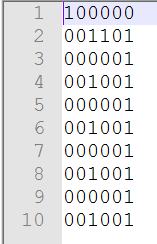
\includegraphics[width=0.68\textwidth]{source/6.png}
								\caption{محتوای فایل \lr{memory.bin}}
								\label{fig:6}
	\end{figure}
	 سپس برای شناساندن این فایل به ماژول، \lr{properties} این تراشه را به صورت زیر به روز می کنیم:
	 \begin{figure}[H]
	 							\centering
	 							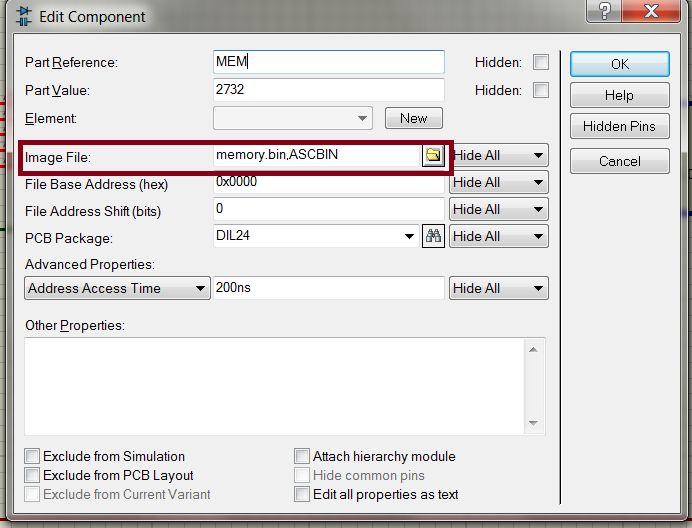
\includegraphics[width=0.68\textwidth]{source/7.png}
	 							\caption{به روز رسانی تنظیمات تراشه 2732}
	 							\label{fig:7}
	 \end{figure}
	 در نهایت توجه داشته باشید که خروجی این حافظه که مشخص کننده دستور بعدی است، به ورودی های ماژول محاسبات \lr{َALU} متصل است. (\ref{fig:2})ماژول فوق در آزمایش شماره 5 پیاده سازی شده است.
\section{تست مدار}
برای بررسی عملکرد و صحت سیستم طراحی شده می خواهیم برنامه محاسبه 10 جمله ابتدایی سری فیبوناچی را پس از بارگذاری در حافظه دستورات اجرا کنیم. این دبناله به صورت زیر تعریف شده است:
 \begin{figure}[H]
 	 							\centering
 	 							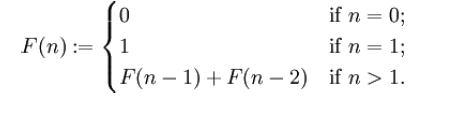
\includegraphics[width=0.68\textwidth]{source/8.png}
 	 							\caption{سری فیبوناچی}
 	 							\label{fig:8}
 \end{figure}
 هم چنین قطعه برنامه زیر ده جمله ابتدایی این سری را در رجیسترهای \lr{R0} و \lr{R1} تولید و می کند، بدین صورت که در هر کلاک، دوجمله انتهایی دنباله تا آن لحظه در ثبات های مذکور ذخیره می شوند.
 \begin{figure}[H]
 	 							\centering
 	 							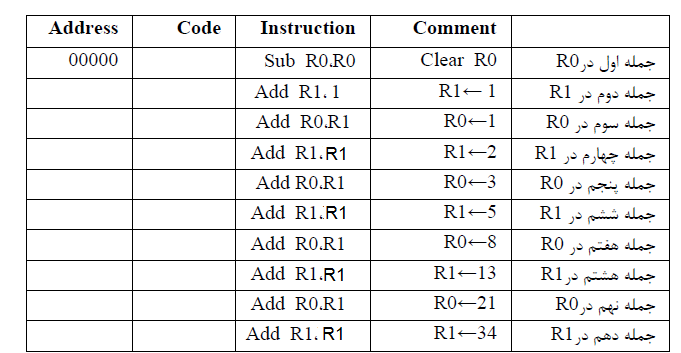
\includegraphics[width=0.68\textwidth]{source/9.png}
 	 							\caption{برنامه محاسبه سری فیبوناچی}
 	 							\label{fig:9}
 \end{figure}
 توجه داشته باشید که کد هر دستور در شکل \ref{fig:6} قابل مشاهده است.
 
 در ادامه وضعیت اجرای مدار در هر کلاک به همراه توضیحات مربوطه آمده اند. در کلیه اشکال، دستور بعدی در قسمت\lr{Memory Output} قابل مشاهده می باشد.
 
 \begin{figure}[H]
  	 							\centering
  	 							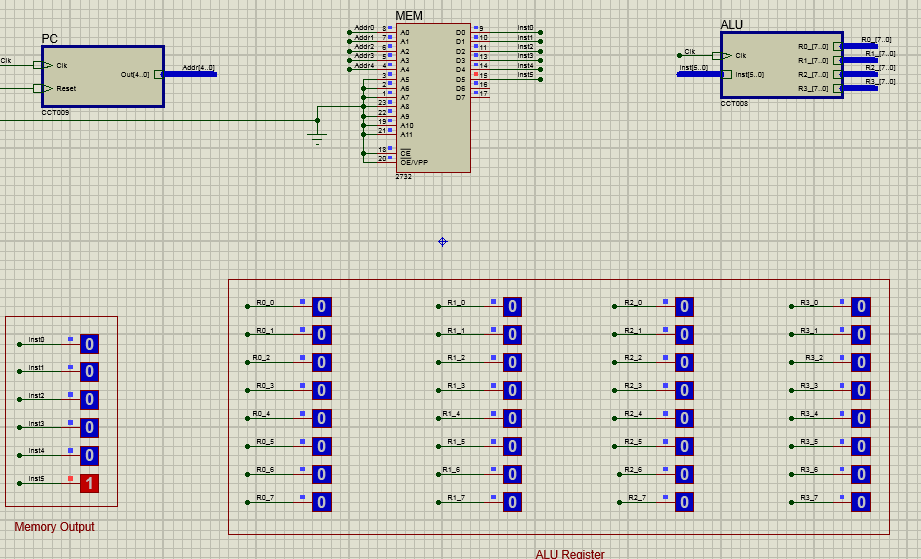
\includegraphics[width=0.68\textwidth]{source/10.png}
  	 							\caption{وضعیت مدار در هنگام شروع}
  	 							\label{fig:10}
 \end{figure}
 \begin{figure}[H]
  	 							\centering
  	 							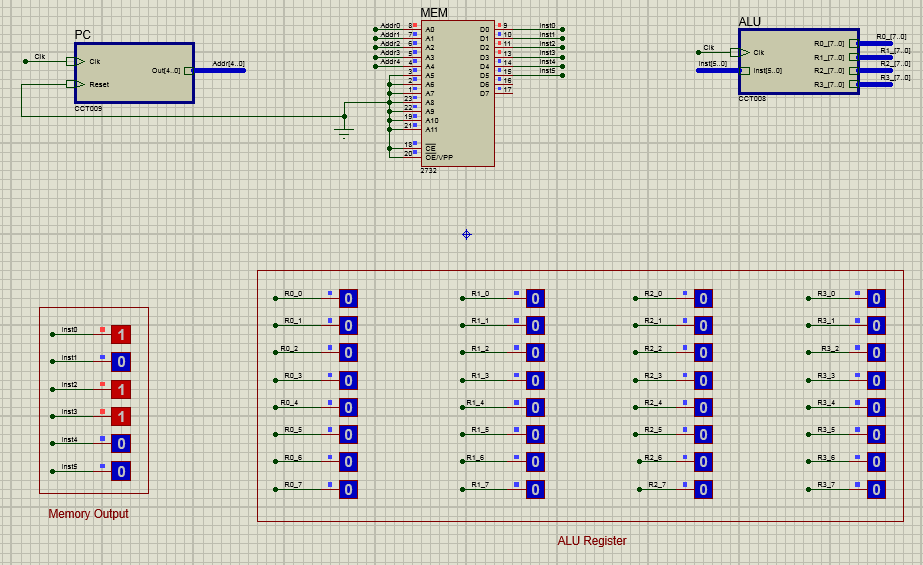
\includegraphics[width=0.68\textwidth]{source/11.png}
  	 							\caption{\lr{Clear R0}}
  	 							\label{fig:11}
 \end{figure}
 \begin{figure}[H]
  	 							\centering
  	 							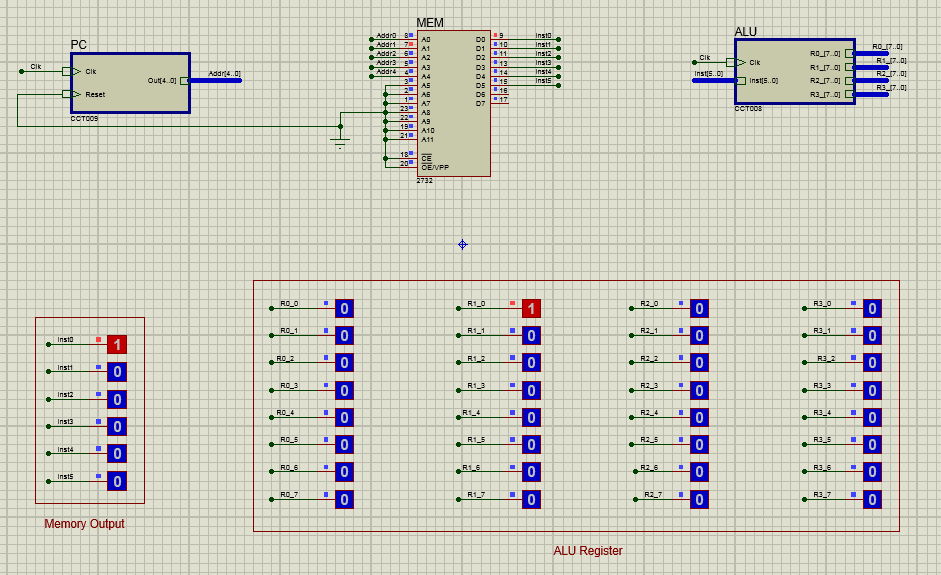
\includegraphics[width=0.68\textwidth]{source/12.png}
  	 							\caption{$R1 \leftarrow 1$}
  	 							\label{fig:12}
 \end{figure}
 
 \begin{figure}[H]
  	 							\centering
  	 							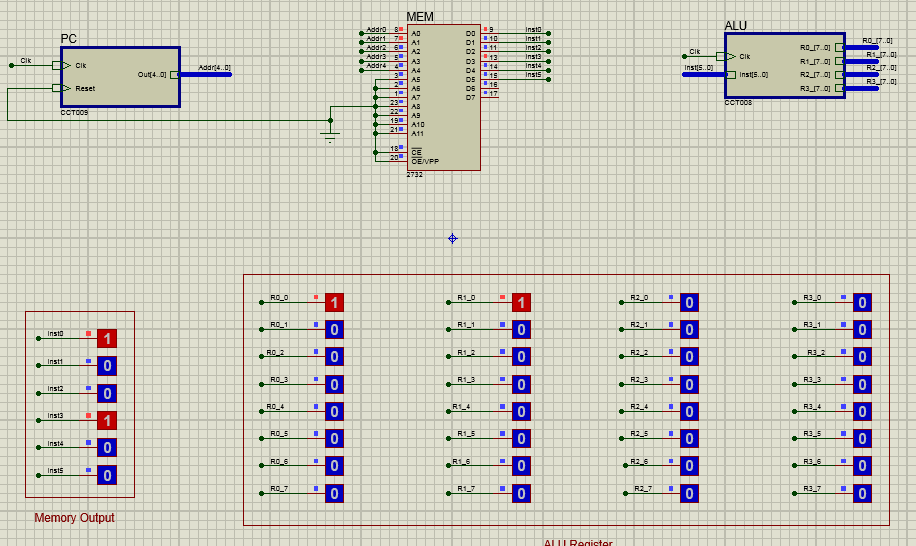
\includegraphics[width=0.68\textwidth]{source/13.png}
  	 							\caption{$R0 \leftarrow 1$}
  	 							\label{fig:13}
 \end{figure}
 \begin{figure}[H]
   	 							\centering
   	 							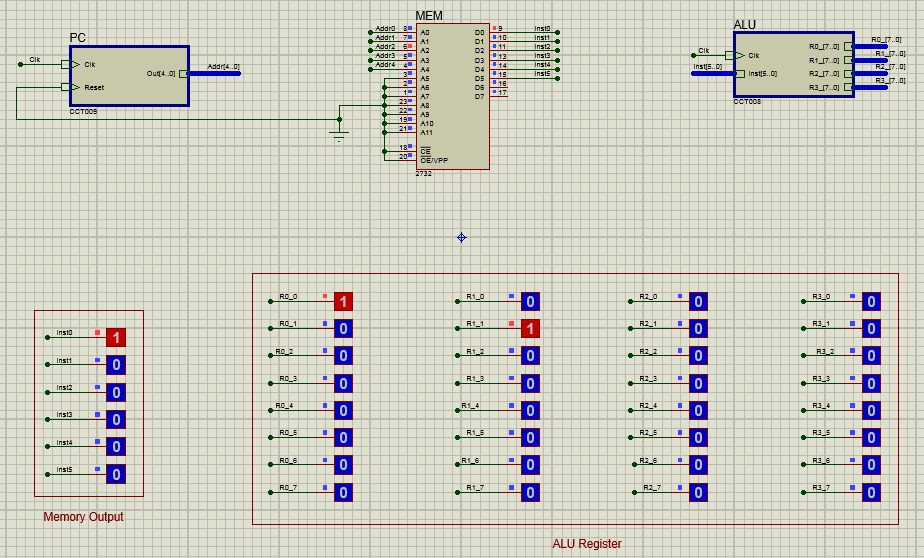
\includegraphics[width=0.68\textwidth]{source/14.png}
   	 							\caption{$R1 \leftarrow 2$}
   	 							\label{fig:14}
  \end{figure}
  \begin{figure}[H]
    	 							\centering
    	 							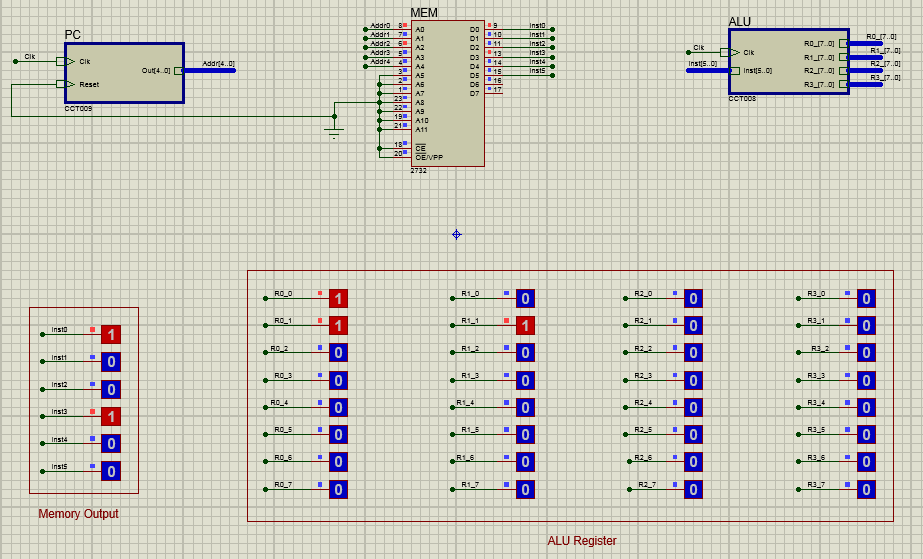
\includegraphics[width=0.68\textwidth]{source/15.png}
    	 							\caption{$R0 \leftarrow 3$}
    	 							\label{fig:15}
   \end{figure}
   \begin{figure}[H]
     	 							\centering
     	 							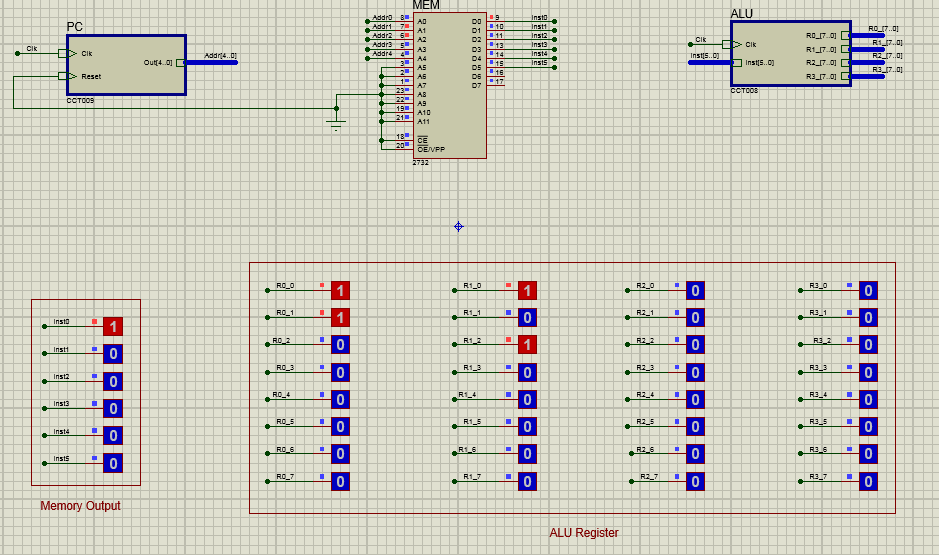
\includegraphics[width=0.68\textwidth]{source/16.png}
     	 							\caption{$R1 \leftarrow 5$}
     	 							\label{fig:16}
    \end{figure}
    \begin{figure}[H]
      	 							\centering
      	 							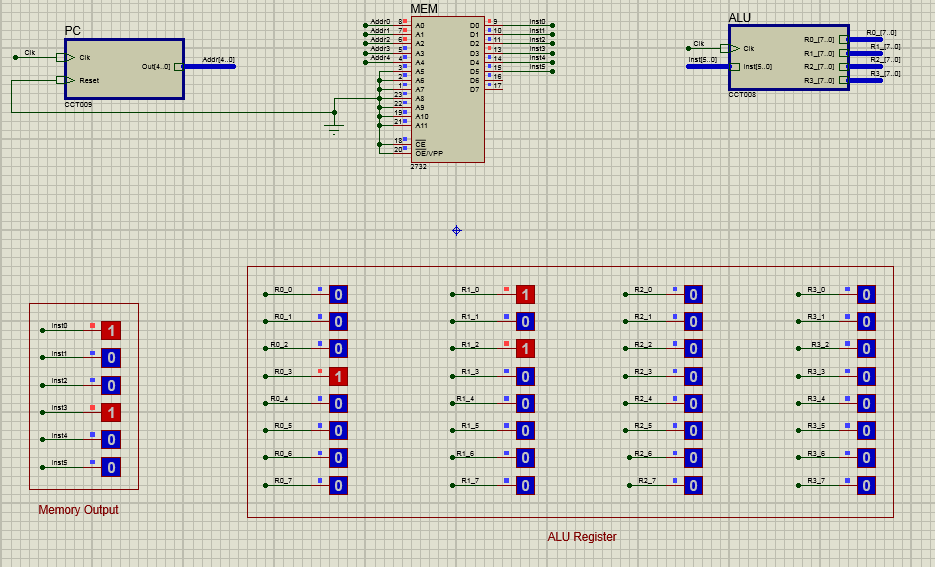
\includegraphics[width=0.68\textwidth]{source/17.png}
      	 							\caption{$R0 \leftarrow 8$}
      	 							\label{fig:17}
     \end{figure}
     \begin{figure}[H]
       	 							\centering
       	 							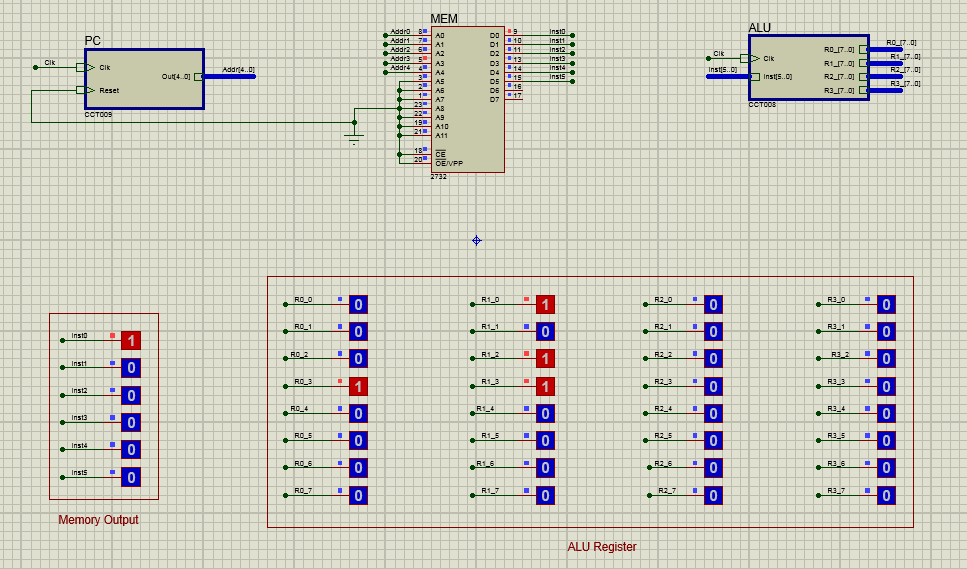
\includegraphics[width=0.68\textwidth]{source/18.png}
       	 							\caption{$R1 \leftarrow 13$}
       	 							\label{fig:18}
      \end{figure}
      \begin{figure}[H]
        	 							\centering
        	 							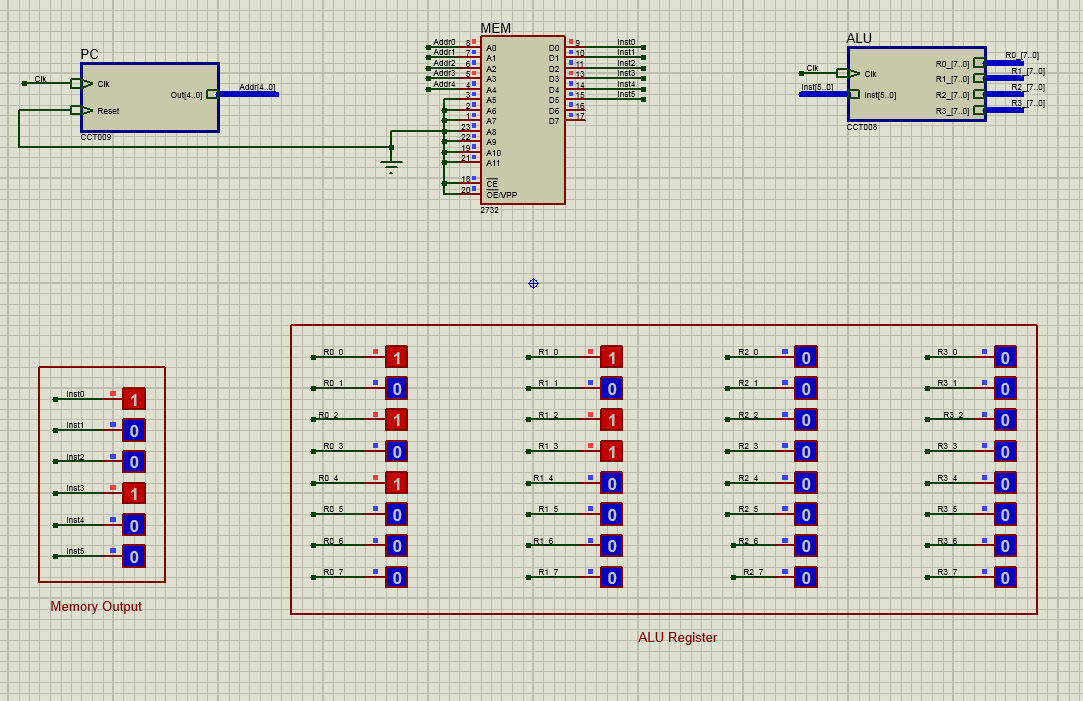
\includegraphics[width=0.68\textwidth]{source/19.png}
        	 							\caption{$R0 \leftarrow 21$}
        	 							\label{fig:19}
       \end{figure}
       \begin{figure}[H]
         	 							\centering
         	 							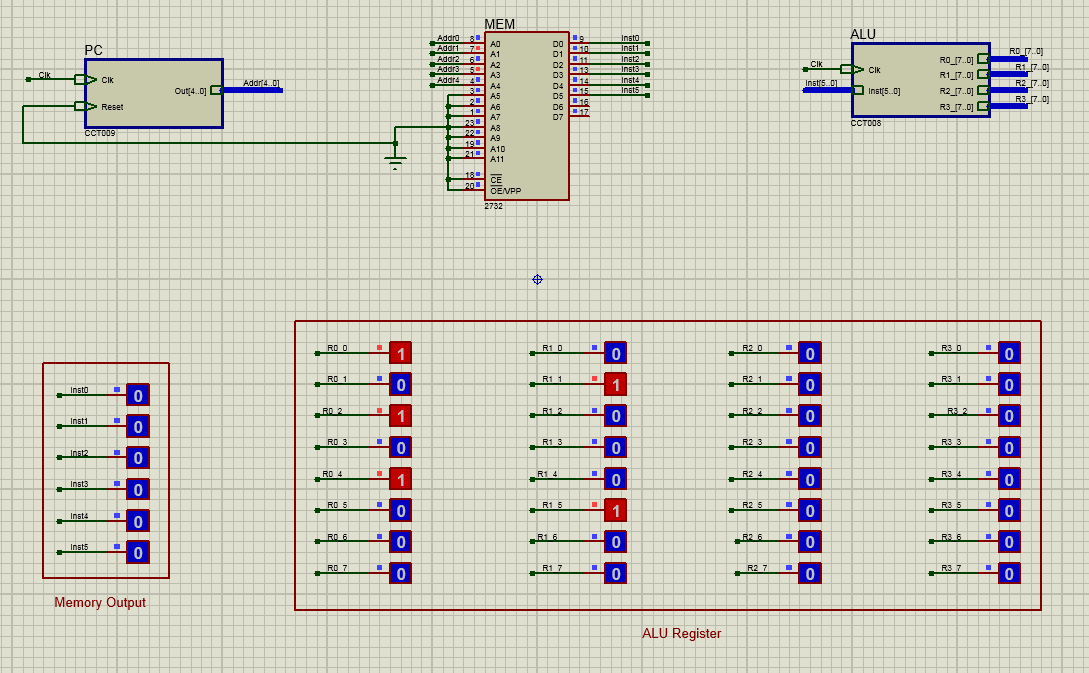
\includegraphics[width=0.68\textwidth]{source/20.png}
         	 							\caption{$R1 \leftarrow 34$}
         	 							\label{fig:20}
        \end{figure} 
 
\end{document}